\documentclass[10pt, conference, compsocconf]{IEEEtran}
\usepackage[usenames,dvipsnames,svgnames,x11names,table]{xcolor}
\usepackage[T1]{fontenc}
\usepackage{amsmath}
\usepackage{amssymb}
\usepackage{tikz}

\begin{document}

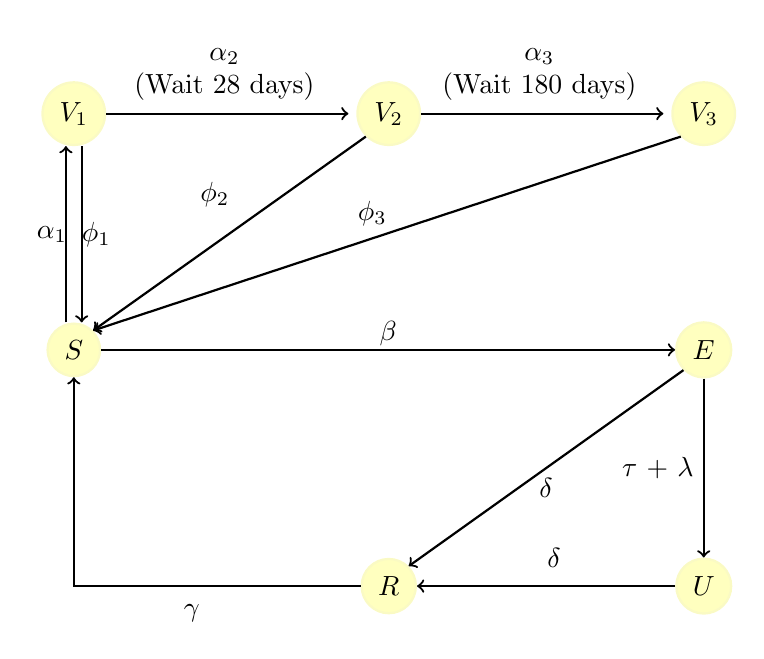
\begin{tikzpicture}[
	block/.style={%
		circle,minimum size=5mm,thick,draw=Yellow!85!Grey!25!,fill=Yellow!25!
	}]
	\node (S) [block] at (-3,0) {$S$};
	\node (V1) [block] at (-3,3) {$V_1$};
	\node (V2) [block] at (1,3) {$V_2$};
	\node (V3) [block] at (5,3) {$V_3$};
	\node (I) [block] at (5,-3) {$U$};
	\node (E) [block] at (5,0) {$E$};
	\node (R) [block] at (1,-3) {$R$};
	\draw[->,thick] ([xshift=-0.1cm]S.north) {} -- node[right,xshift=-0.5cm] {$\alpha_1$} ([xshift=-0.1cm]V1.south);
	\draw[->,thick] (V1.east) {} |- node[above,xshift=1.5cm] {\begin{tabular}{c} $\alpha_2$ \\ (Wait 28 days) \end{tabular}} ([xshift=-0.1cm]V2.west);
	\draw[->,thick] (V2.east) {} |- node[above,xshift=1.5cm] {\begin{tabular}{c} $\alpha_3$ \\ (Wait 180 days) \end{tabular}} ([xshift=-0.1cm]V3.west);
	\draw[->,thick] ([xshift=0.1cm]V1.south) {} -- node[left,xshift=0.5cm] {$\phi_1$} ([xshift=0.1cm]S.north);
	\draw[->,thick] (V2.south west) {} -- node[right,xshift=-0.5cm,yshift=0.5cm] {$\phi_2$} (S.north east);
	\draw[->,thick] (V3.south west) {} -- node[right,xshift=-0.5cm,yshift=0.25cm] {$\phi_3$} (S.north east);
	\draw[->,thick] (S.east) {} -- node[below,yshift=0.5cm] {$\beta$} (E.west);
	\draw[->,thick] (E.south) -- node[left] {$\tau$  + $\lambda$} (I.north);
	\draw[->,thick] (I.west) {} -- node[above,xshift=0.1cm,yshift=0.1cm] {$\delta$} (R.east);
	\draw[->,thick] (E.south west) {} -- node[below] {$\delta$} (R.north east);
	\draw[->,thick] (R.west) {} -| node[below,xshift=1.5cm,yshift=-0.1cm] {$\gamma$} (S.south);
\end{tikzpicture}

\end{document}